%\section{Paradigmi}

Gli elementi grafici e funzionali sono solo una parte dell'architettura del software di Metarace.
%
Un'altra componente importante dell'architettura di Metarace è che sfrutta il paradigma della programmazione guidata dagli eventi.
%
Nella programmazione guidata dagli eventi il flusso del programma è determinato da eventi esterni ad esso, come l'input di un utente o come un messaggio arrivato da un server.
%
Infatti Metarace ha una struttura capace di rispondere agli eventi avviati dal server ma anche agli eventi innescati dall'utente.
%
Il software presenta un'interfaccia utente che permette al giocatore di avviare una partita e, dato che esistono diverse tipologie di partite, di scegliere la tipologia di gara a cui partecipare.
%
L'insieme degli eventi che possono verificarsi è stato scelto in fase di elaborazione ed è costituito da 13 eventi.
%
Parte del mio lavoro è stato la progettazione e l'implementazione di 9 di questi, che sono: PlayEvent, AvailableRacesEvent, JoinEvent, PlayerJoinedEvent, StartingGridEvent, AnotherPlayerJoinedEvent, CountdownEvent, RaceEvent, LeaderboardEvent.

%\section{Model - View - Controller (MVC)}
\section{L'architettura di Metarace}

Un videogioco è un applicativo che è particolarmente adatto alla divisione a strati.
%
Infatti l'architettura di Metarace può essere divisa in vari strati che si occupano del suo funzionamento.
%
È possibile individuare lo strato della Logica Implementativa, lo strato del Network, lo strato dell'Interfaccia Grafica e lo strato dell'Interfaccia Utente (UI).

\begin{description}
    \item[Lo strato della Logica Implementativa] è composto da tutti gli script che permettono il funzionamento dell'applicazione.
    \item[Lo strato del Network] permette di comunicare da e verso il server e di tradurre queste comunicazioni in istruzioni per lo strato della Logica Implementativa.
    \item[Lo strato dell'Interfaccia Grafica] è composto dall'engine di gioco e da tutti gli elementi che vengono renderizzati a schermo.
    \item[Lo strato della UI] permette di catturare l'input dato dall'utente e di tradurlo in rispettivi eventi di gioco.
\end{description}

\begin{figure}[!ht]
    \centering
    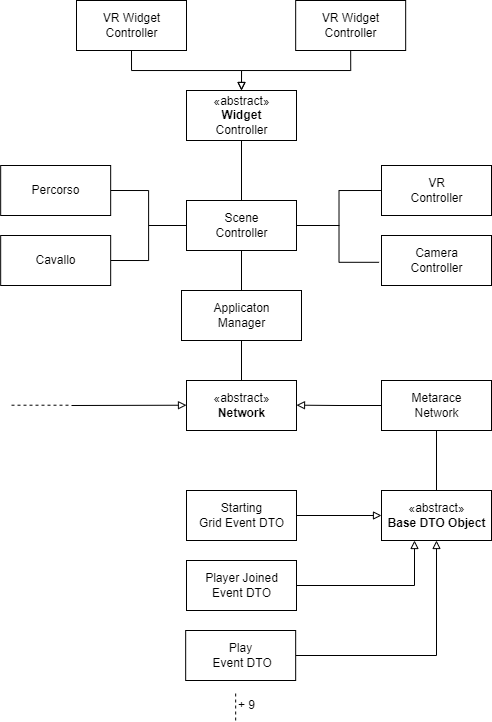
\includegraphics[width=12cm]{figure/Modello_di_Dominio_Metarace.drawio.png}
    \caption{Modello di Dominio parziale per Metarace}
    \label{img:Dominio}
\end{figure}

    \subsection{Progettazione guidata dalle responsabilità}

    Nella progettazione guidata dalle responsabilità gli oggetti software sono considerati come dotati di responsabilità, di ruoli e di collaborazioni.
    %
    Sulla base del modello di dominio  parziale mostrato in Figura \ref{img:Dominio} vengono assegnate le responsabilità di ciascun oggetto.

    Le responsabilità sono di due tipi: \textit{Responsabilità di fare} e \textit{Responsabilità di conoscere}.
    %
    Un importante tipo di responsabilità di fare è quella del pattern \textit{Creator}.
    %
    La maggiorparte delle responsabilità di questo tipo sono state assegnate all'oggetto \textit{Application Manager}.  
    %
    Questo è anche dovuto dal fatto che nel momento in cui il gioco viene fatto partire, un attore deve essere già in scena per poter instanziare tutti gli altri Actor.
    %
    Questo attore è proprio l'\textit{Application Manager}.

    Un'altro importante pattern da seguire quando si assegnano le responsabilità è il pattern \textit{Low Coupling}.
    %
    Questo pattern punta a cercare il progetto che abbia il minor livello di accoppiamento.
    %
    Per tenere l'accoppiamento basso in Metarace è stato sfruttato uno strumento offerto da Unreal Engine: i delegates.

    I delegates permettono di chiamare funzioni di oggetti C++ in modo generico e type-safe \cite{UDelegates}.
    %
    Un delegate può essere legato dinamicamente ad una funzione di un oggetto scelto e permette di eseguire questa funzione in un momento futuro senza che il chiamante debba conoscere il tipo dell'oggetto chiamato.
    %
    Questo strumento riduce di molto l'accoppiamento in quanto in questo modo due oggetti possono collaborare senza conoscersi.

    \subsection{L'\textit{Application Manager}}

    L'Application Manager è l'unica classe già presente in scena durante la prima chiamata alla funzione \textit{Begin Play}.
    %
    In Unreal Engine è possibile posizionare una classe C++ nel mondo di gioco attraverso la creazione di un Blueprint sulla base di essa.
    %
    Allo stesso modo all'interno di una classe C++ è possibile avere dei riferimenti ad altri Blueprint basati sempre su classi C++.
    %
    Infatti, Unreal Engine permette di creare questo tipo di riferimenti attraverso il template di classe \textit{TSubclassOf<T>}.

    \begin{lstlisting}[caption = Sezione dell'header file della classe ApplicationManager dove vengono referenziate altri Blueprint basati su classi C++]
#include ...

UCLASS()
class Metarace AMetaraceApplicationManager : public AActor
{
    [...] //Costruttore di classe, funzione BeginPlay e Tick

protected:
    UPROPERTY(Category=TableController, EditAnywhere, BlueprintReadWrite)
    TSubclassOf<AMetaraceSceneController> SceneControllerBP;
    UPROPERTY(Category=TableController, EditAnywhere, BlueprintReadWrite)
    TSubclassOf<AMetaraceNetworkActor> NetworkActorBP;

private:
    UPROPERTY()
    AMetaraceSceneController* SceneController = nullptr;
    UPROPERTY()
    AMetaraceNetworkActor* NetworkActor = nullptr;
};        
    \end{lstlisting}

    Nella funzione \textit{Begin Play} viene messo in pratica il pattern \textit{Create} per gli oggetti SceneController e NetworkActor:

    \begin{lstlisting}[caption = Sezione del file source dell'Application Manager dove vengono creati gli oggetti SceneController e NetworkActor]
void AMetaraceApplicationManager::BeginPlay()
{
    Super::BeginPlay();

    UWorld* World = GetWorld();
    if(!World) { return; }

    FActorSpawnParameters SpawnParams;
    if(SceneControllerBP)
    {
        SceneController = World->SpawnActor<AMetaraceSceneController>(
            SceneControllerBP, GetTransform(), SpawnParams);
    }
    if(NetworkActorBP)
    {
        NetworkActor = World->SpawnActor<AMetaraceNetworkActor>(
            NetworkActorBP, GetTransform(), SpawnParams);
        NetworkActor->Initialize();
    }

    \end{lstlisting}

    L'ApplicationManager si occupa anche di creare i Bind per tutti i delegate visto che già ha i riferimenti a tutti gli oggetti che li utilizzano.

    \begin{lstlisting}[firstnumber=22, caption = Sezione del file source dell'Application Manager dove viene formato il Bind dei delegates, label = {alg:bindDelegate}]

    if(SceneController && NetworkActor)
    {
        SceneController->OnWantToSendMessage.
            BindUObject(NetworkActor, 
                &MetaraceNetworkActor::SendMessage);
        SceneController->WidgetController->OnWantToSendMessage.
            BindUObject(NetworkActor, 
                &AMetaraceNetworkActor::SendMessage);

        NetworkActor->OnAvailableRacesFormatsEventDelegate.
            BindUObject(SceneController,
                &AMetaraceSceneController::ShowAvailableRaceFormats);
        NetworkActor->OnPlayerJoinedEventDelegate.
            BindUObject(SceneController,
                &AMetaraceSceneController::PlayerJoined);
        NetworkActor->OnStartingGridEventDelegate.
            BindUObject(SceneController,
                &AMetaraceSceneController::StartingGrid);
        NetworkActor->OnRaceEventDelegate.
            BindUObject(SceneController,
                &AMetaraceSceneController::InitRace);
        NetworkActor->OnCountdownEventDelegate.
            BindUObject(SceneController,
                &AMetaraceSceneController::ShowCountDown);
        NetworkActor->OnAnotherPlayerJoinedEventDelegate.
            BindUObject(SceneController,
                &AMetaraceSceneController::AnotherPlayerJoined);
        NetworkActor->OnLeaderboardEventDelegate.
            BindUObject(SceneController,
                &AMetaraceSceneController::OnLeaderboardEvent);
    }
}        
    \end{lstlisting}

    Lo SceneController possiede un delegate perché a gara finita deve poter inviare il file \textit{Json} per l'evento \textit{RaceFinischedEvent} verso il server.
    %
    Il WidgetController anche possiede un delegate perché deve poter inviare messaggi verso il server dato che è lui che si occupa degli eventi \textit{PlayEvent} e \textit{JoinEvent}.
    %
    NetworkActor possiede inoltre un delegate per ogni evento che deve gestire e viene creato il Bind con lo SceneController per delegare quest'ultimo a eseguire la logica implementativa.

    Dopo l'esecuzione della funzione \textit{Begin Play} l'ApplicationManager non viene più chiamato.

    \subsection{Lo \textit{SceneController}}

    Lo \textit{SceneController} è la classe implementata per permettere di interfacciarsi con lo strato di Logica Implementativa e con lo strato dell'Interfaccia Utente.
    %
    A questa classe sono state assegnate le responsabilità di conoscere gli oggetti più importanti del livello di gioco: il percorso di gara e i cavalli. 
    %
    Infatti, si occupa dello \textit{spawn} dei cavalli dei giocatori e del settaggio delle loro variabili.
    %
    Inoltre si occupa della creazione delle classi WidgetController, CameraController e VRController.
    %
    Lo SceneController crea l'istanza del WidgetController in base alla presenza o meno del VR connesso al computer.
    %
    Questo può essere controllato grazie alla libreria offerta da Unreal Engine \textit{UHeadMountedDisplayFunctionLibrary}.

    \begin{figure}[!ht]
        \centering
        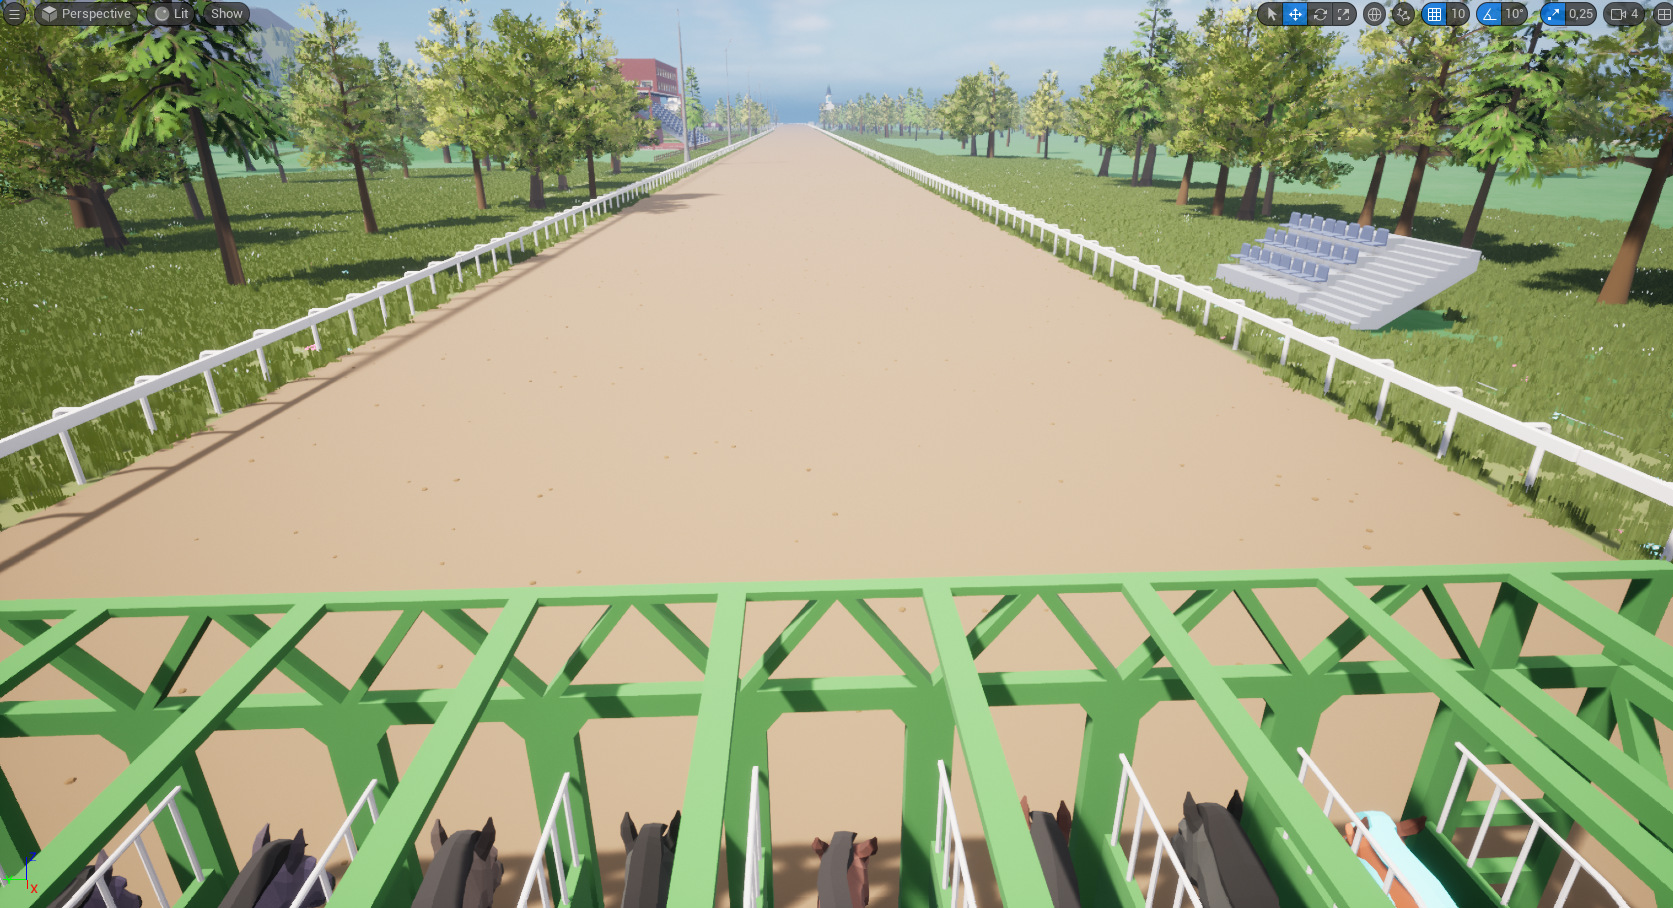
\includegraphics[width=12cm]{figure/HorseView2Cropped.png}
        \caption{Vista dall'inizio del percorso, dopo che lo SceneController ha fatto comparire i cavalli}
    \end{figure}

    \begin{lstlisting}[caption = Sezione del source della classe SceneController dove viene fatto il controllo per sapere se il giocatore indossa un visore]
void AMetaraceSceneController::BeginPlay()
{
    Super::BeginPlay();
    UWorld* World = GetWorld();
    if(!World) { return; }

    IsInVR = UHeadMountedDisplayFunctionLibrary::IsHeadMountedDisplayConnected();

    if(IsInVR)
	{
		if(BP_VRController)
		{
			VRController = World->SpawnActor<AVRMetaraceController>(BP_VRController, GetTransform(), SpawnParams);
		}
		if(BP_VRWidgetController)
		{
			WidgetController = World->SpawnActor<AMetaraceVRWidgetController>(
				BP_VRWidgetController, GetTransform(), SpawnParams);
		}
    }else
    {
        if(BP_CameraController)
		{
			CameraController = World->SpawnActor<AMetaraceCameraController>(
				BP_CameraController, GetTransform(), SpawnParams);
		}
		if(BP_3DWidgetController)
		{
			WidgetController = World->SpawnActor<AMetaraceWidgetController>(
				BP_3DWidgetController, GetTransform(), SpawnParams);
		}
    }
    [...]
}        
    \end{lstlisting}

    Lo SceneController implementa tutte le funzioni che sono collegate con i delegate del NetworkActor.

    \subsection{Il \textit{WidgetController}}

    Il \textit{WidgetController} è la classe implementata per permettere di gestore la creazione, l'interazione e la visualizzazione dei Widget.
    %
    I Widget sono delle strutture offerte da Unreal Engine con cui è possibile creare e far comparire l'Interfaccia Utente.
    %
    Questi oggetti sono il punto di accesso al sistema offerto al giocatore.
    %
    Infatti, permettono di mostrare testi e pulsanti (più in generale interfacce UI) con cui il giocatore può interagire.

    La classe WidgetController è astratta perché esistono due implementazioni in base a se il giocatore è in VR oppure no. 
    %
    Infatti i Widget hanno un comportamento molto diverso nei due casi.
    %
    Se il giocatore non indossa un visore VR i widget saranno soltanto degli oggetti 2D che verranno mostrati a schermo.
    %
    Se invece il giocatore indossa un visore VR i widget dovranno essere istanziati come oggetti 3D nel mondo di gioco.
    %
    In entrambi i casi le funzionalità dei singoli widget dovranno essere mantenute.

    Ho creato i Widget partendo dalla classe C++.
    %
    Infatti può essere istanziato sulla base di una classe che estende la classe di Unreal Engine \textit{UUserWidget}.
    %
    Sulla base di questa classe va creato un Blueprint di tipo Widget (un particolare tipo di Blueprint) in cui inserire la classe come istanza di Widget. 
    %
    È possibile definire degli elementi del Widget (testuali o interagibili come dei bottoni) all'interno del codice e collegarli con le variabili nell'istanza Blueprint con lo specificatore UPROPERTY con l'opzione \textit{meta = (BindWidget)}.
    %
    Questa specificazione crea un bind automatico con la variabile all'interno del Bluprint ma quest'ultima deve avere necessariamente lo stesso nome della corrispettiva nello script (in questo caso \textit{StartButton}).
    %
    È mostrato il codice relativo alla classe che implementa il Widget per il pulsante \textit{Start}, chiamata \textit{StartMenuWidget}:

    \begin{lstlisting}[caption = File header della classe StartMenuWidget]
#include ...

DECLARE_DYNAMIC_MULTICAST_DELEGATE_OneParam(FDelegateOnClickStartRaceEventUI , bool, toShow);

UCLASS()
class Metarace UStartMenuWidget : public UUserWidget
{
	GENERATED_BODY()
	
public:
	UPROPERTY(EditAnywhere, BlueprintReadWrite, meta = (BindWidget))
	class UButton* StartButton;

	UPROPERTY()
	class AMetaraceBaseWidgetController* WidgetController = nullptr;

	virtual void NativeConstruct() override;

	UFUNCTION()
	void onStartClicked();

	FDelegateOnClickStartRaceEventUI Delegate_OnClickStartRaceEventUI;
	
};
    \end{lstlisting}

    Per definire la funzione da chiamare quando un bottone viene premuto dall'utente bisogna fare creare un legame con la funzione scelta (che ho chiamato in questa classe \textit{onStartClicked}).
    %
    Questo si può chiamare con la funzione \textit{AddUniqueDymanic} come mostrato di seguito.
    %

    Nella funzione OnStartClicked viene mostrato l'esecuzione del delegate che si occupa di inviare il file Json al server. 

    
    \begin{lstlisting}[ caption = {File source classe StartMenuWidget}, label= {alg:StartWidget} ]
#include ...

void UStartMenuWidget::NativeConstruct()
{
    Super::NativeConstruct();

    StartButton->OnClicked.AddUniqueDynamic(this, 
        &UStartMenuWidget::onStartClicked);
}

void UStartMenuWidget::onStartClicked()
{
    if(WidgetController && 
        WidgetController->OnWantToSendMessage.IsBound())
    {
        FJsonObject o;
        o.SetStringField("event", "Play");
        WidgetController->OnWantToSendMessage.
            Execute(Utility::JsonToString(o));	
    }
}
    \end{lstlisting}

    La classe \textit{BaseWidgetController} definisce le funzioni seguenti:

    \begin{lstlisting}[caption=File header della classe astratta BaseWidgetController]
#include ...
DECLARE_DELEGATE_OneParam(FOnWantToSendMessage, const FString&);

UCLASS()
class Metarace AMetaraceBaseWidgetController : public AActor
{
    GENERATED_BODY()
    [...] //Constructor, BeginPlay e Tick Function
public:
    virtual void ShowStartUI() {};
    virtual void ShowRaceFormats(TArray<URaceFormatObject*> Formats) {};
    virtual void RemoveRaceFormats() {};
    virtual void UpdateTimer() {};
    virtual void ShowCountdown(int Seconds) {};
    virtual void ShowRaceWidget() {};
    virtual void ShowLeaderboard(TArray<ULeaderboardObjectDTO*> LeaderboardLines) {};

    FOnWantToSendMessage OnWantToSendMessage;
};
    \end{lstlisting}

    Nel caso in cui il giocatore non stia collegato con un visore si possono far comparire i Widget come delle immagini 2D a schermo.
    %
    Ho perciò utilizzato le funzioni seguenti per questo scopo:

    \begin{lstlisting}[caption = Crezione di istanza di Widget con StartMenuWidget come esempio]
StartMenuWidget = CreateWidget<UStartMenuWidget>(GetWorld(), BP_StartWidget);
StartMenuWidget->WidgetController = this;
    \end{lstlisting}

    \begin{lstlisting}[firstnumber=4, caption = Aggiunta di Widget al Viewport]
StartMenuWidget->AddToViewport(0);
    \end{lstlisting}

    Mentre nel caso in cui il giocatore stia collegato con un visore per la realtà virtuale i Widget sono stati inseriti come Widget Component all'interno di un Blueprint comune.
    %
    In questo modo è possibile renderizzarli come delle immagini all'interno dell'ambiente 3D di gioco, come mostrato in figura \ref{img:WidgetVR}. 

    \begin{figure}[!t]\label{img:WidgetVR}
        \centering
        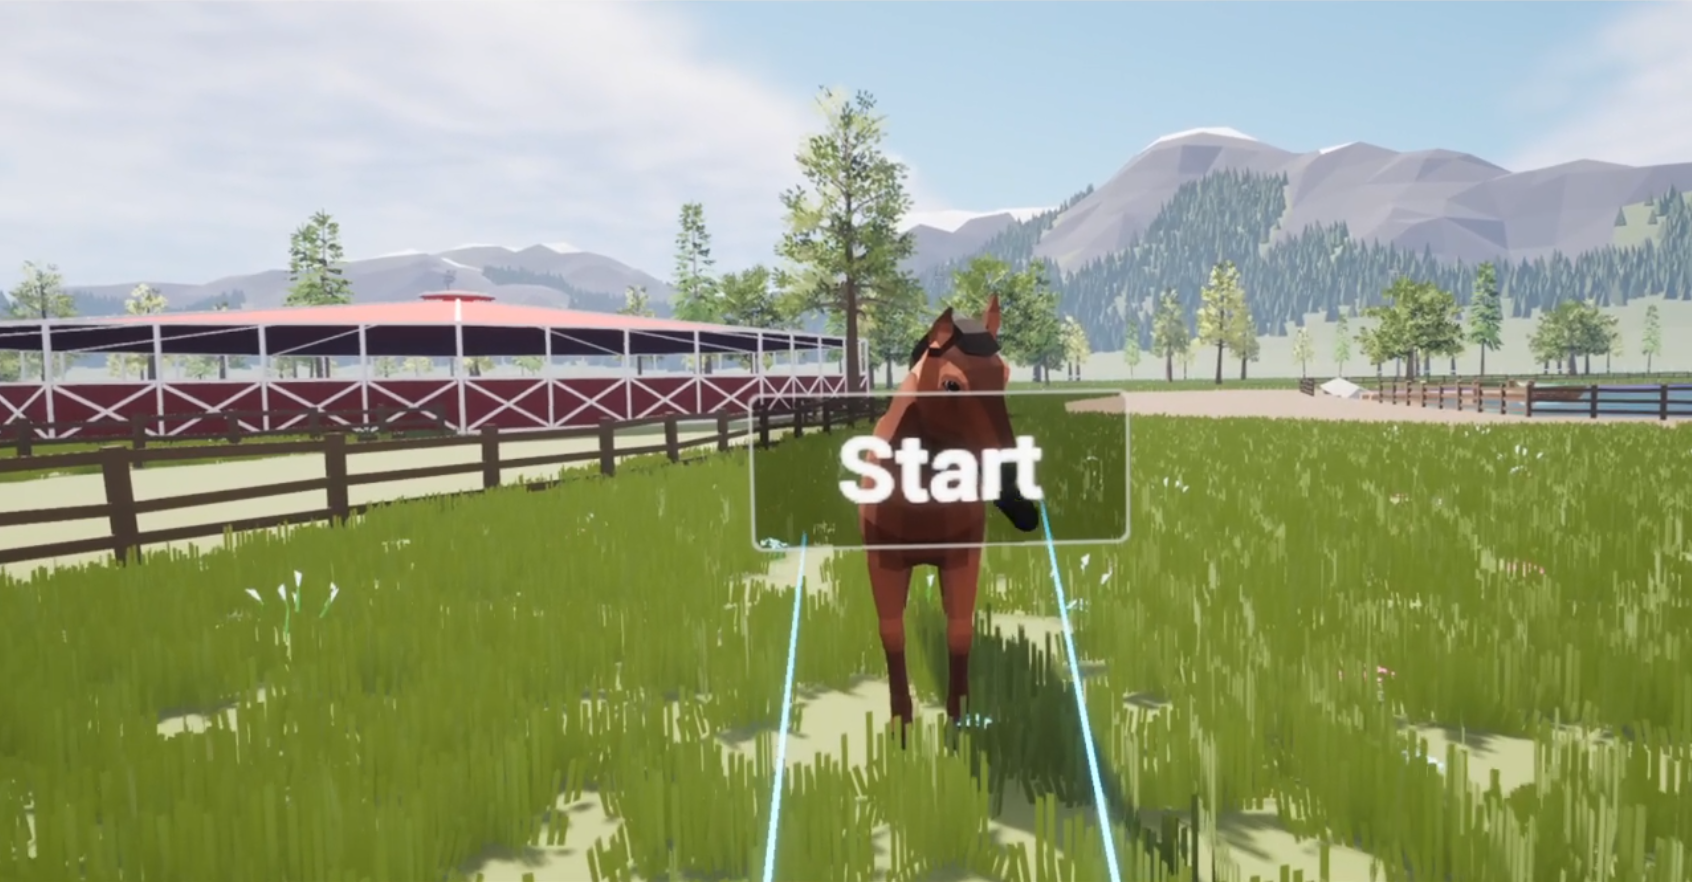
\includegraphics[width=12cm]{figure/StartMenuVRWidget2.png}
        \caption{Widget renderizzato in 3D per la modalità VR}
    \end{figure}

    Per questo scopo si utilizzano le funzioni per lo spawn degli Actor e si cerca successivamente il Widget Component al loro interno in modo da ottenere la classe Widget con le funzionalità cercate.
    %
    È possibile interagire con il Widget mentre si è in modalità VR puntando il joystick verso il pulstante e premento il tasto corrispondente all'interazione.
    %
    Il codice seguente mostra l'utilizzo di queste funzioni per il VRWidget \textit{StartMenuWidget}:

    \begin{lstlisting}[caption = Creazione Widget VR per la classe \textit{StartMenuWidget}]
VRStartMenu = World->SpawnActor<AActor>(BP_VRStartMenu, SpawnTransform, SpawnParams);
UWidgetComponent* WidgetComponent = VRStartMenu->FindComponentByClass<UWidgetComponent>();
StartMenuWidget = Cast<UStartMenuWidget>(WidgetComponent->GetWidget());
StartMenuWidget->WidgetController = this;
    \end{lstlisting}

    È possibile infine mostrare o nascondere il Blueprint desiderato attraverso la libreria \textit{ESplateVisibility} che permette di scegliere tra \textit{Visible}, \textit{Hidden} e altre opzioni.

    Degno di nota è infine lo strumento \textit{UListView} che permette di inserire a tempo di esecuzioni un numero variabile di Widget all'interno di un altro Widget, potendo perciò creare dei Widget a cascata anche a tempo di esecuzione.
    %
    Equivalente è lo strumento \textit{UTileView}.
    %
    I due strumenti sono stati utilizzati rispettivamente per renderizzare il Widget per la classifica finale e per renderizzare la griglia di pulsanti con cui è possibile scegliere il formato di gara a cui partecipare.

    \subsection{Il {CameraController}}

    Il \textit{CameraController} è la classe implementata per permette di gestire il movimento delle camere e di cambiare visione da una camera ad un'altra in base alle esigenze.
    
    Sebbene potrebbe presentare funzioni simili al VRController, queste due classi non sono state pensate per avere le stesse funzioni perché il CameraController non è un sostituto dell'implementazione VR.
    %
    Infatti le telecamere non servono unicamente per renderizzare il mondo di gioco al vista del giocatore, ma possono renderizzare il mondo di gioco anche come texture di oggetti all'interno del mondo stesso.
    %
    L'implementazione di questa classe quindi può essere scalata per utilizzare l'output delle telecamere per simulare una televisione o un altro dispositivo digitale per far vedere al giocatore immerso nel mondo di gioco un canale televisivo con in onda la gara stessa.

    \begin{figure}[!ht]\label{img:CineCameraActor}
        \centering
        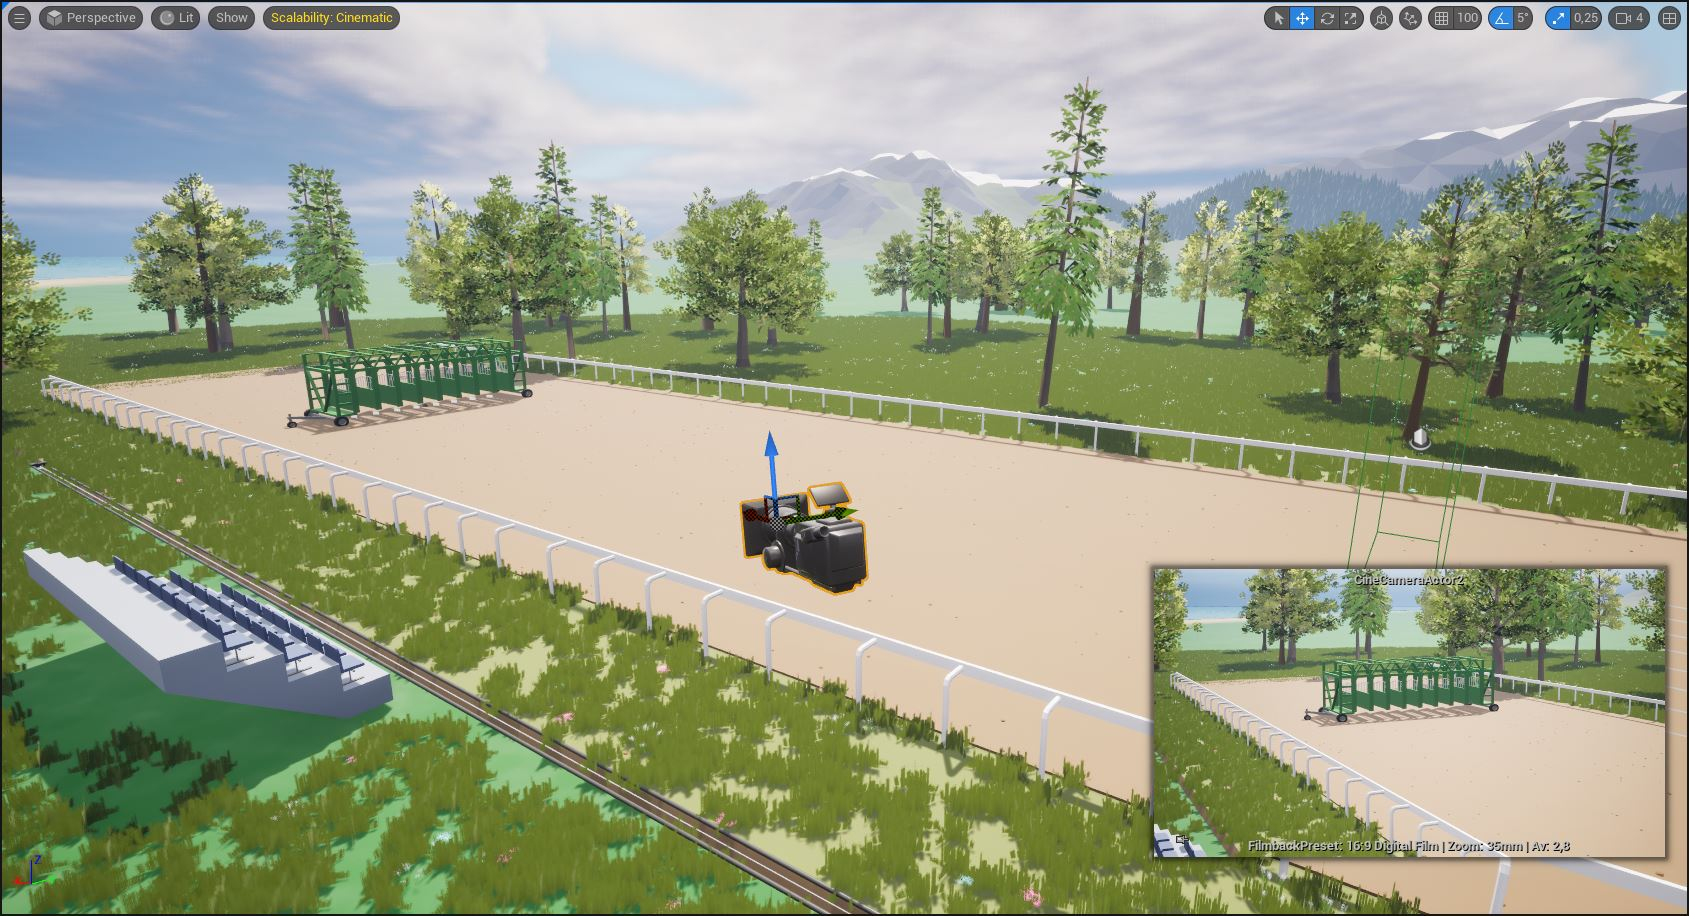
\includegraphics[width=12cm]{figure/CameraActor.JPG}
        \caption{CineCameraActor che riprendere la griglia di partenza}
    \end{figure}

    Per le camere di gioco sono state scelte le \textit{CineCameraActor} perché permettono di tenere al centro dell'inquadratura un attore nel mondo di gioco.
    %
    Questa caratteristica è particolarmente utile per ricreare l'effetto di una camera ferma in un punto nello spazio che gira su se stessa per inquadrare il soggetto, come accade nelle trasmissioni televisive che riprendono le competizioni.
    %
    È stato usato anche un oggetto CameraRigRail per ottenere un binario cinematografico per ricreare l'effetto di una telecamera che segue i cavalli.
    %
    Questo strumento è composto da una Spline e da un modello 3D per far visualizzare allo sviluppatore la posizione della camera lungo di essa.
    %
    La CameraRigRail si è dimostrata particolamente comoda in questo contesto perché visto che i cavalli si muovono lungo una Spline si è potuto impostare il carrello della stessa lunghezza del percorso.
    %
    A quel punto è stato possibile passare il valore della distanza a cui si trova il cavallo lungo la spline al carrello per posizionare la camera alla stessa altezza dei cavalli.
    %
    La position lungo il rail è standardizzata tra 0 e 1 perciò basta passare il valore di output della Timeline, per questo scopo è stata usata la funzione seguente:

    \begin{lstlisting}{caption = Funzione per aggiornare la posizione della CineCamera lungo il RigRail}
void AMetaraceCameraController::UpdateCameraPositionOnSpline(float TimelineValue)
{
    CameraRail->CurrentpPositionOnRail = TimelineValue;
}
    \end{lstlisting}

    All'interno del percorso sono stati inseriti degli oggetti \textit{ATriggerBox} per poter cambiare telecamere al raggiungimento di questi trigger, nella Figura \ref{img:CineCameraActor} ne è mostrato uno.
    %
    Gli oggetti \textit{ATriggerBox} permettono di impostare degli eventi \textit{Overlap} che permettono di cambiare camera quando i cavalli raggiungo un punto lungo il percorso.

    \begin{lstlisting}[caption = {Chiamata per l'aggiunta di una funzione all'evento overlap di un \textit{TriggerBox}}]
StartRaceTriggerBox->OnActorEndOverlap.AddDynamic(this, 
    &AMetaraceCameraController::OnStartTriggerExit);
    \end{lstlisting}

    È possibile passare da una camera ad un'altra chiamando la funzione \textit{SetViewTargetWithBlend} che offre la possibilità di avere un movimento fluido per il cambio da un'inquadratura ad un'altra su una base di un valore temporale passato in input.

    \begin{lstlisting}[caption = Funzione per impostare la telecamera per la vista dell'utente]
void AMetaraceCameraController::OnStartTriggerExit(AActor* This, AActor* Other)
{
    if(CineCamera)
    {
        PlayerController->SetViewTargetWithBlend(
            CineCamera, 3); 
    }
}
    \end{lstlisting}

    \subsection{Il \textit{VRController}}

    La classe \textit{VRController} si occupa di implementare le chiamate dello \textit{SceneController} quando il giocatore ha eseguito l'accesso al gioco tramite un visore per la realtà virtuale.

    \begin{figure}[!ht]
        \centering
        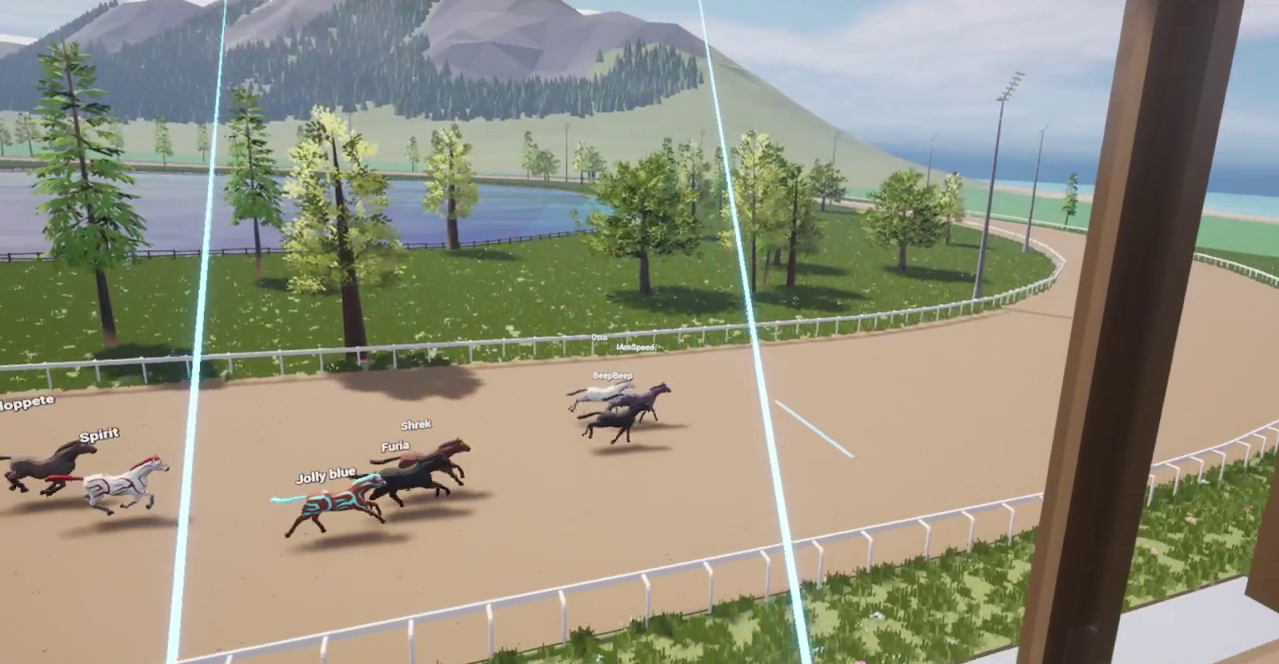
\includegraphics[width=12cm]{figure/VRVisuale.png}
        \caption{Visuale della gara in VR da una posizione appositamente creata}
    \end{figure}

    Il giocatore in questa modalità oltre che poter interagire con i widget può assistere alla gara dagli spalti e da posizioni lungo il percorso appositamente create per lo scopo.
    %
    Ad esempio ho creato una sala interna di un edificio che affaccia sul percorso da dove è possibile avere una visuale della gara.

    Questa classe possiede un \textit{TArray} di posizioni che implementano una logica di ordinazione.
    %
    Le posizioni sono ordinate e posizionate lungo il percorso che fanno i cavalli in modo che il giocatore può scorrerle avanti e indietro.
    %
    Le funzioni che implementano questa logica sono:
    
    \begin{lstlisting}[ caption = Funzioni per teleportare il giocatore lungo le posizioni per assistere alla gara]
void AVRMetaraceController::NextPosition()
{
    int32 temp = CurrentPosition+1;
    if(!PlayerPositions.IsEmpty() && temp<PlayerPositions.Num() && temp>=0)
    {
        if(Player)
        {
            Player->TeleportTo(
                PlayerPositions[temp]->GetActorLocation(),
                PlayerPositions[temp]->GetActorRotation());
            CurrentPosition = temp;
        }
    }
}

void AVRMetaraceController::PrevPosition()
{
    int32 temp = CurrentPosition-1;
    if(!PlayerPositions.IsEmpty() && temp<PlayerPositions.Num() && temp>=0)
    {
        if(Player)
        {
            Player->TeleportTo(PlayerPositions[temp]->GetActorLocation(),
                PlayerPositions[temp]->GetActorRotation());
            CurrentPosition = temp;
        }
    }
}
    \end{lstlisting}

% Lo metto qui invece che nell'implementazione perché per ora non c'è un'implementazione ma questa cosa è stata comunque nella fase di progettazione

% L'ingegniere prende scelte

% Mettere molti grafici